\documentclass[a4paper,10pt]{article} 

\usepackage[utf8]{inputenc} 


\usepackage{textcomp}           % Extra Symbole (Grad Celsius etc.)
\usepackage{amssymb,amsmath}    % Schöne Formeln (AMS = American Mathematical Society)
\usepackage{graphicx}           % Bilder und Seitenränder
\usepackage{subcaption}			% captions for subfigures
\usepackage{booktabs}           % Schönere Tabellen
\usepackage{colortbl}           % Farbige Tabellen

%\usepackage{tcolorbox}			% schöne bunte Boxen
\usepackage{mathtools}			% \mathclap für ordentliche \underbrace-			environments
\usepackage{geometry}			% Pagelayout mit \newgeometry, \restoregeometry
\usepackage{float}
\usepackage{wrapfig}
\usepackage{enumitem}
\usepackage{float}
\usepackage{braket}
\usepackage{caption}
\usepackage[version=4]{mhchem}
\usepackage{siunitx}
\usepackage{enumitem}

\DeclareSIUnit\year{yr}
\graphicspath{{./img/}}
\newcommand*{\dif}{\mathrm{d}}

\bibliographystyle{unsrtnat}

\renewcommand{\k}{\mathbf{k}}
\begin{document}
\begin{titlepage}
 \begin{center}
	\Large{Advanced laboratory class 2}
	\end{center}
	\begin{center}
	 \LARGE{\textbf{FP2 - Photometric measurements of the dissociation of manganese oxalate}}
	\end{center}
	
	\begin{center}
	
	\large Marco \textsc{Canteri} \\
	marco.canteri@student.uibk.ac.at\\
	\large Johannes \textsc{Willi} \\
	johannes.willi@student.uibk.ac.at
	\end{center}
	
	\begin{center}
	\vspace{1cm}
	Innsbruck, \today
	\vspace{2cm}
	\end{center}
	
	\begin{center}
	
\includegraphics[scale=0.4]{img/uibk} 
	\end{center}

\end{titlepage}
\begin{abstract}
In this experiment we measured the dissociation rate constants of manganese(III) oxalate at three different temperatures by means of photometric measurements. We monitored the absorption of the solution for 20 minutes in order to extract the dissociation rate. Moreover, we estimated the activation energy and the frequency factor of the dissociation.
\end{abstract}
\section{Introduction}
Photometric measurements provide a great tool to study chemical reaction, since it is possible to measure concentrations of a solution during a reaction. Therefore it is possible to study the time evolution and the speed of a chemical reaction. In this work we took advantage of this method and we studied the dissociation of manganese(III) oxalate. We determined the reaction rate of the dissociation for three different temperature: 23 °C, 30 °C, and 35 °C, by monitoring the reaction for around 20 minutes. We measured the absorption of the solution and we related the intensity of the laser with the concentration of manganese(III) oxalate, which allowed us to study the speed of such reaction. Furthermore, we studied the energy activation of the reaction and the frequency factor from the Arrhenius equation.
\section{Theory}
We want to study the dissociation of manganese(III) oxalate. This molecule is obtained from potassium permanganate (\ce{KMnO4}) which react with oxalic acid (\ce{C2H2O4}) with the following reaction
\begin{center}
\ce{2MnO4- + 5H2C2O4 + 6H+ -> 2Mn^2+ + 10CO2 + 8H2O }
\end{center} 
where the manganese goes from oxidation state of (VII) to (II). This reaction is composed of multiple step, but we are interested in the last one, where the manganese change the oxidation state from (III) to (II), i.e. the dissociation of manganese(III) oxalate that we want to study. We can study this step neglecting the others because this is the slowest one \cite{manganese}, therefore the overall reaction is indeed dominated by this dissociation. This reaction is the following \cite{taube}
\begin{center}
\ce{[Mn(C2O4)3]3- + 2H2O- -> [Mn(C2O4)2(H2O)2]2- +CO2 + CO2- }
\end{center} 
It is worth noticing that the the \ce{CO2} created is gaseous and therefore during the reaction it is released. Hence, the reaction is non reversible, since the carbon dioxide needed for the reverse reaction is lost.\\
As already said, we study the dissociation by means of absorption, we can estimate the concentration of manganese(III) oxalate based on how much light it absorbs. The intensity of the absorbed light is given by the Lamber-Beer law
\[I = I_0 10^{-\varepsilon c d },\]
where $I_0$ is the intensity before the absorption, $\varepsilon$ is the molar absorption coefficient, $c$ is the concentration, and $d$ is the length of optical path. We can rewrite this equation to get the concentration
\begin{equation}\label{absorbance}A \equiv \log\left(\frac{I_0}{I}\right) = \varepsilon c d,\end{equation}
where we have also defined the absorbance $A$. This relationship holds as long as the concentration is not high.\\
We are interested in the speed of the reaction, in general for a reaction \ce{aA + bB -> cC} the speed is defined as the change in concentration over the time, mathematically
\[v = -\frac{1}{a}\frac{\partial[A]}{\partial t} = -\frac{1}{b}\frac{\partial[B]}{\partial t} = \frac{1}{c}\frac{\partial[C]}{\partial t}.\]
The reaction rate law correlates the speed with the concentrations of the molecules
\begin{equation}\label{speed}v = k [A]^m [B]^n,\end{equation}
where $k$ is the rate constant that we want to measure and $m+n$ is the order of the reaction, which cannot be found theoretically, but it is determined experimentally. For our experiment, the dissociation of manganese(III) oxalate can be approximated with a first order reaction, therefore the equation \eqref{speed} can be written as
\[v = -\frac{\partial[A]}{\partial t} = k [A].\]
This differential equation can be solved relatively easily by the method of separation of variables
\[\frac{d[A]}{[A]} = -kdt \implies [A] = [A]_0 e^{-kt},\]
whereas $[A]_0$ is the concentration of $A$ at time 0. By taking the natural logarithm we can linearize the equation
\[\ln([A]) = -kt + \ln([A]_0).\]
It is clear now that is possible to find $k$ with a fit done on this line. The concentration of $[A]$ over time is found with the absorbance of equation \eqref{absorbance}, the factors $\varepsilon$ and $d$ do not really play a role in the fit, in fact with the property of logarithms it is easy to show that these factors will only change the intercept of the line, not the slope $k$ that we want to measure.\\
Finally we also want to measure the activation energy $E_a$ of the reaction, this quantity can be related with $k$ via the Arrhenius equation
\[k = \mathcal{A} e^{-\frac{E_a}{RT}},\]
where $\mathcal{A}$ is called the frequency factor, $R$ is the universal gas constant, and $T$ is the temperature. The linearized equation is
\[\ln(k) = \ln(\mathcal{A}) - \frac{E_a}{RT}.\]
Therefore, if we plot $\ln(k)$ as a function of the inverse of the temperature, the frequency factor and the activation energy can be found.

\section{Experiment setup and procedure}
The experiment setup is quite simple, as light source we used a mercury gas lamp whose output is filtered at 520 nm. The light is then absorbed by our solution placed in a cuvette, and it is measured with a Polytec i-trometer. The data are acquired with the software \emph{BWSpec V 4.0.}.\\
For the experiment we used three different solutions:
\begin{itemize}
	\item Manganese sulfate \ce{MnSO4} 0.2 mol/L
	\item Oxalic acid \ce{C2H2O4} 0.2 mol/L
	\item Potassium permanganate \ce{KMnO4} 0.02 mol/L
\end{itemize} 
Before proceeding with the measurements we took a spectrum of pure water and of potassium permanganate. Then we prepared the mixture at room temperature (23 C°), we mixed in a flask 1 mL of manganese sulfate and 7 mL of oxalic acid. Finally we triggered the reaction by adding 2 mL of potassium permanganate, at this point we have also started the chronometer to record the time of the reaction. Then we poured the mixture in a cuvette and we placed it in front of the laser. We took measurement approximately every minute for twenty minutes. \\
The measurements at 30 °C and 35 °C were trickier, we prepared the same mixture as before with the same procedure, but we keep everything at fixed temperature with a thermalized bath. Between the measurements we kept moving the cuvette between the bath and in front of the laser such that the mixture was kept thermalized. Unfortunately we failed this task for the measurement at 30 °C, where for the first ten minutes we did not put the cuvette back in the bath, so the data points in this case are not ideal.
\section{Data analysis}
\begin{figure}[H]
\centering
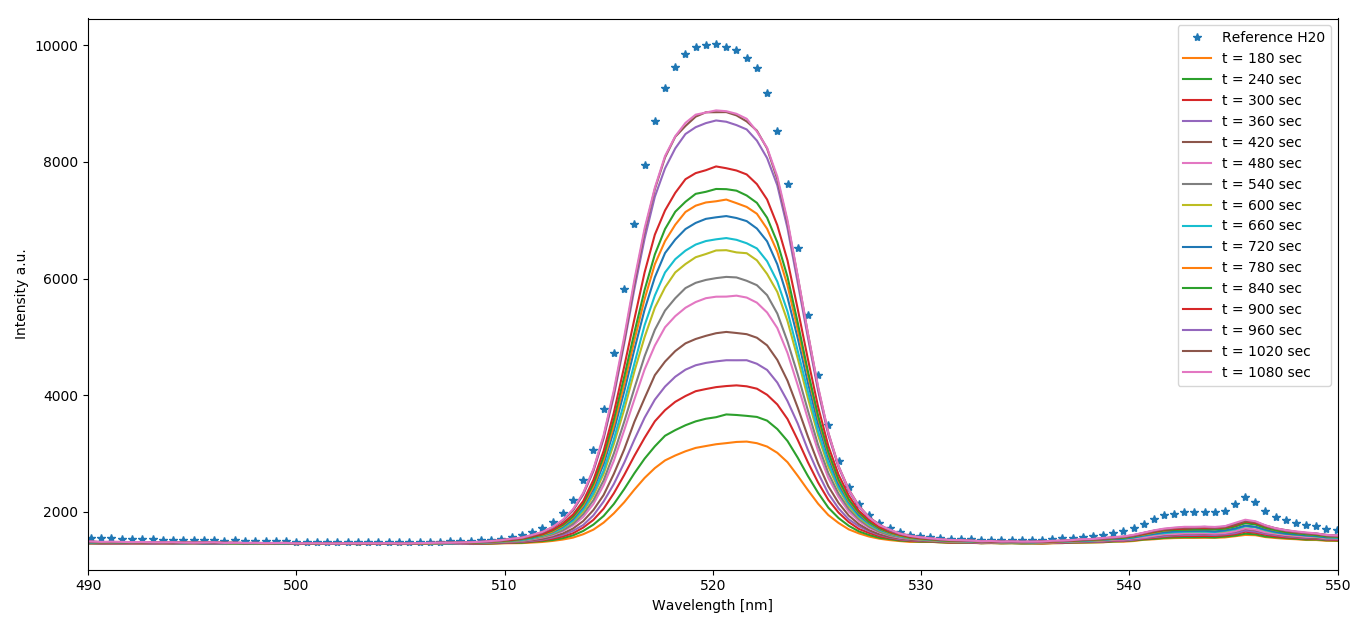
\includegraphics[width=\textwidth]{spectrum30}
\caption{Acquired spectrum for mixture at 30 °C}\label{spectrum}
\end{figure}
An example of acquired data is in figure \ref{spectrum}, we can see the peak at around 520 nm. The longer we wait the higher is the peak, which means that less light is absorbed, as expected. 
As intensity $I$ we calculated the maximum of the peak, then we calculated the absorbance $A$ with equation \eqref{absorbance}, where as $I_0$ we used the maximum of the peak for the reference of water. Moreover, we subtracted the spectrum of potassium permanganate in order to remove the offset that can be seen in figure \ref{spectrum}. We did the same for the data at 23 °C and 35°C. Then we calculated the natural logarithm of $A$ and plotted as a function of time. This is shown in figure \ref{fit}. The lines for the lower temperatures are regular, apart from a point at 300 s for the line of 23 °C, this is due a problem during the measurement, in fact its spectrum is flat. The point relative at 35 °C are quite noisy and apparently random. We are not sure about what happened during these measurements, a possibility is that we placed the cuvette very fast and not always perfectly aligned, so the path length through the cuvette, which we assume to be constant, may in fact not be constant at all. 
\begin{figure}[H]
\centering
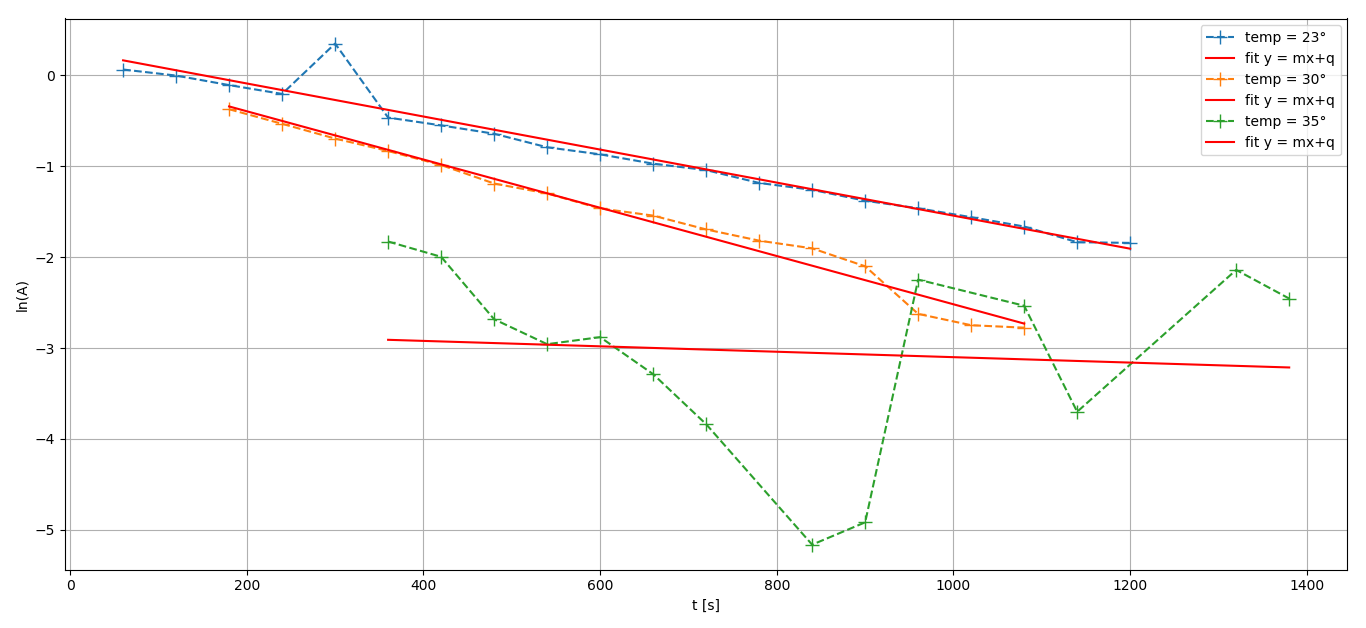
\includegraphics[width=\textwidth]{fit}
\caption{Natural logarithm of the absorbance $A$ for our three different temperature}\label{fit}
\end{figure}
The results of the fits for $k$ are reported in the following table
\begin{table}[H]
\centering
\begin{tabular}{c|c}
 Temperature [°C] & k [$\text{s}^{-1}$] \\
  \hline
  23 & $0.0018\pm 0.0001$ \\
 
   30 & $0.0026\pm 0.0001 $ \\
  
  35 & $0.0003\pm  0.0009$\\
  \hline
\end{tabular}
\end{table} 
the relative error of the last fit is very high since the data are not really in a straight line. Nevertheless, we can notice that the rate constant raise with the temperature as expected. The literature data available are \cite{k}: $k = 0.001$ $\text{s}^{-1}$ at 30 °C, and $k = 0.00028$ $\text{s}^{-1}$ at 20 °C. The rate we measured are not fully compatible with this literature value.\\
For the activation energy we plotted the logarithm of $k$ as a function of $1/T$ and we did a fit as described in the second section. This plot can be found in figure \ref{energy}. From the fit we obtained the value $E_a = -103 \pm 104$ kJ/mol, and for the frequency factor $\mathcal{A} = 1.8\cdot 10^{-21}\pm7.5\cdot 10^{-20}$ $\text{s}^{-1}$. The errors are huge, since the uncertainty on $k$ was large too. The literature value \cite{k} of the activation energy is $E_a = 81588.0$ J/mol which is obviously not compatible with our result. Indeed, we even have a different sign. However in order to have a better result we also fitted a line with the data at lower temperatures. The plot is in figure \ref{energy2}, with only two points is not possible to have an error on the parameters, but the values are $E_a = 40379$ J/mol and $\mathcal{A} = 24080$ $\text{s}^{-1}$ which are more similar to the literature value. Anyway, since we only have two-three data points, our fit cannot be very good either way, an analysis from such little data is sure to be relatively bad. For the frequency factor we did not find a literature value. 
\begin{figure}[H]
\centering
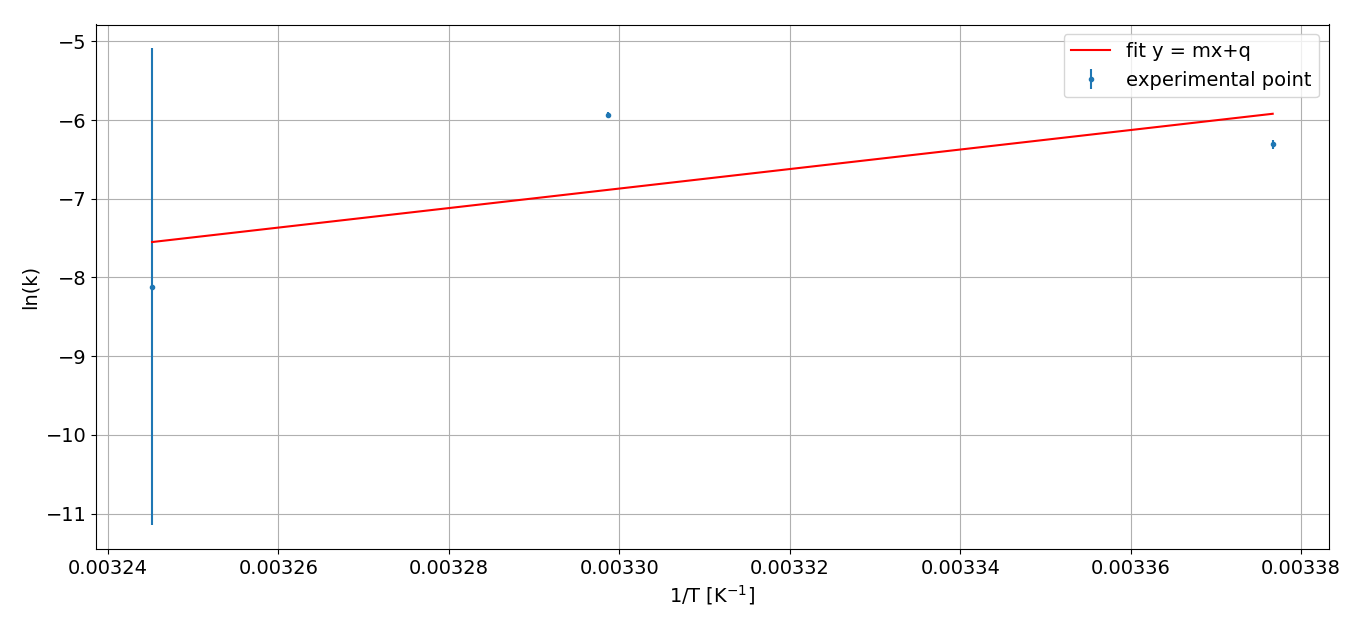
\includegraphics[width=\textwidth]{energy}
\caption{Fit for the activation energy and frequency factor}\label{energy}
\end{figure}
\begin{figure}[H]
\centering
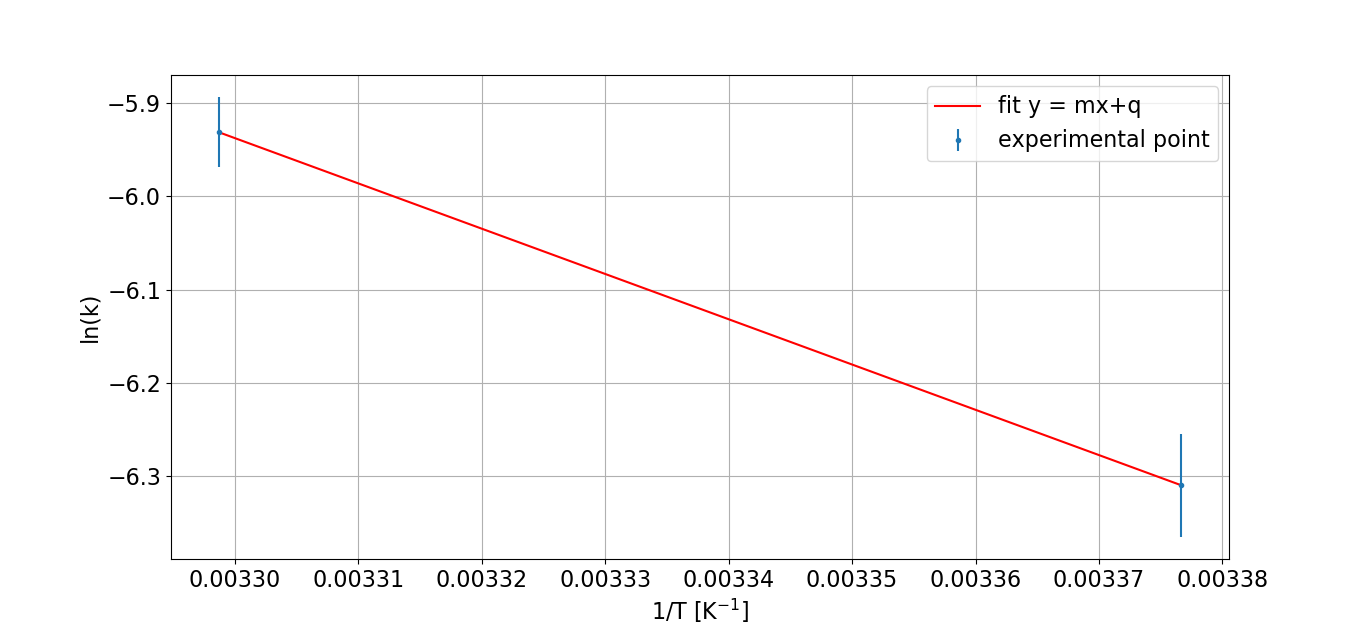
\includegraphics[width=\textwidth]{energy2}
\caption{Fit for the activation energy and frequency factor without the point at 35 °C}\label{energy2}
\end{figure}
\section{Summary and conclusion}
In this experiment we measured the dissociation rate constant of manganese(III) oxalate at three different temperatures. We had some problems with the data took at temperature 35 °C, it is possible that something went wrong with the measurements, for instance we were moving the cuvette between the bath and the place in front of the laser very fast, so likely every time the cuvette was not in the same exact position. The large error of this measurement has propagated to the latter analysis, causing some troubles in the estimation of the activation energy and of the frequency factor whose results are not satisfactory. 


\section{Questions - Marco Canteri}
\begin{enumerate}[label=\alph*)]
	\item The colour of potassium permanganate arises from a ligand metal charge transfer, i.e. an electron is promoted from the highest energy state of the bond manganese-oxygen to a $d$ state of the manganese. This transaction absorbs yellow light, thus we see the complementary colour, purple.
	\item In order to ease the study of a molecule, it is common to use the Born–Oppenheimer approximation, which separates the electronic states from the nuclei motion. A typical energy curve is in figure \ref{frank}, where there are depicted two electronic potential curves. For each of this curve the vibrational state of the nuclei are represented for different energy level. In a molecule several type of transition can occur, it can change electronic state, vibrational state, rotational state, a so on. Everyone of this transition manifests as an absorption line in the spectrum. In particular the Franck-Condon principle is related to vibronic transitions which are transitions where the molecule change both electronic and vibrational state. The principle, in its quantum formulation, states that a vibronic transition has an higher probability of happening if the overlap integral between the two wavefunctions of the states is greater. Basically the electronic transition are instant with respect to the motion of the nuclei, which it is slow compared to the electrons. Therefore the vibronic transition are vertical, that is the positions of the nuclei do not change during the electronic transition.
	\begin{figure}[H]
	\centering
	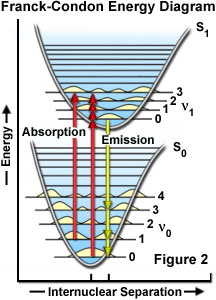
\includegraphics[width=0.4\textwidth]{frank.jpg}
	\caption{Energy diagram for a molecule, the vibrational state can be approximated with an harmonic oscillator, while the electronic curves are given by the morse potential}\label{frank}
	\end{figure}

	\item Carbon-14 undergoes $\beta$ decay: \ce{^14C -> ^14N + e- + \nu_e-}, which is a first order reaction. For a first order reaction it holds that $t_{1/2} = \ln(2)/k$, where $t_{1/2}$ is the half-life, and k is the rate constant. With this formula we can calculate immediately 
	\[k= \frac{\ln(2)}{t_{1/2}} \simeq 1.21\cdot10^{-4} \,\,\text{years}^{-1}.\]
	The concentration of a first order reaction follows a exponentially decay $A = A_0 e^{-kt}$, imposing $A/A_0 = 0.72$ we can calculate the time at which $A$ was 28\% lower the $A_0$
	\[t = -\frac{1}{k}\ln\left(\frac{A}{A_0}\right) \simeq 2715  \,\,\text{years}\]
	\item The chemical reaction is \ce{A -> B + C}, if this is a first order reaction we can write the usual reaction law as
	\begin{equation}\label{firstorder} v = -\frac{d[A]}{dt} = k_a [A] \implies [A] = [A]_0 e^{-k_a t},\end{equation}
	where $[A]_0$ is the concentration at time 0. The rate can be also expressed with the concentration of $B$ and $C$, in the case of $B$ we have
	\[v = \frac{d[B]}{dt} = k_b [A].\]
	This equation can be solved by using as $[A]$ what we found in equation \eqref{firstorder} and solving the differential equation by separating the variables
	\[\frac{d[B]}{dt} = k_b [A]_0 e^{-k_a t} \implies d[B] = k_b [A]_0 e^{-k_a t}\,dt,\]
	we can easily integrate in both side of this equation and we obtain
	\[[B] = -\frac{k_b [A]_0 e^{-k_a t}}{k_a} + C\]
	where $C$ is a constant which can be found by imposing the condition that at time 0 the concentration of $[B]$ is zero. In conclusion we have
	\[[B] = \frac{k_b [A]_0}{k_a}(1-e^{-k_a t}). \]
	Similarly we can get the equation for the concentration of $[C]$ which differs from $[B]$ only by the factor $k_c$ instead of $k_b$
	\[[C] = \frac{k_c [A]_0}{k_a}(1-e^{-k_a t}).\]
	A plot of the evolution of these concentrations is in figure \ref{plot}
	\begin{figure}[H]
\centering
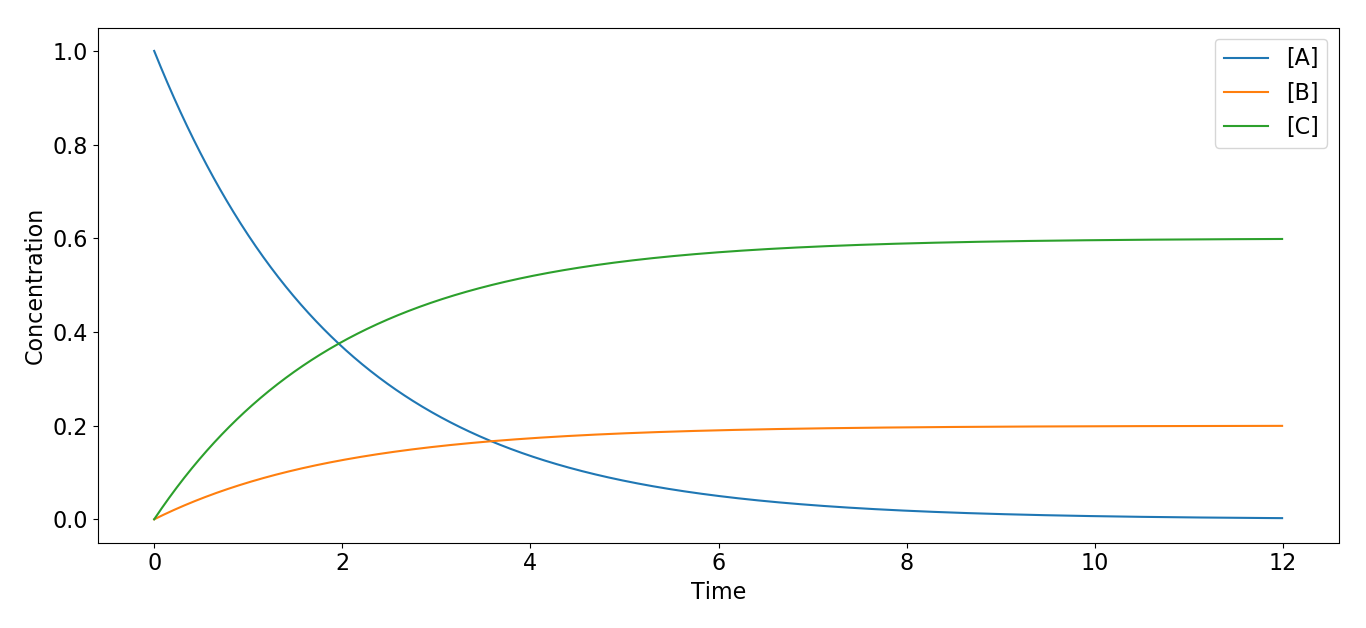
\includegraphics[width=\textwidth]{question}
\caption{Concentration of reactant and products in the reaction \ce{A -> B + C}, where $k_c > k_b$}\label{plot}
\end{figure}
\end{enumerate}


\section{Questions - Johannes Willi}
\begin{enumerate}
\item Potassium permanganate (KMnO$_4$) is purple because of an electronic transition. More precisely, a charge 
transfer reaction inside the molecule takes place via a photon(s) that promotes an electron from the highest energy molecular orbital in one of the MnO bonds to an empty d-orbital of the manganese. This transfer has an energy equivalent 
of roughly 570 nm, which the human eye perceives as yellow. So "yellow" photons are absorbed, leaving the complimentary color of yellow, which is purple.
\item Consider the following diagram of a molecules energy levels
\begin{figure}[H]
\centering
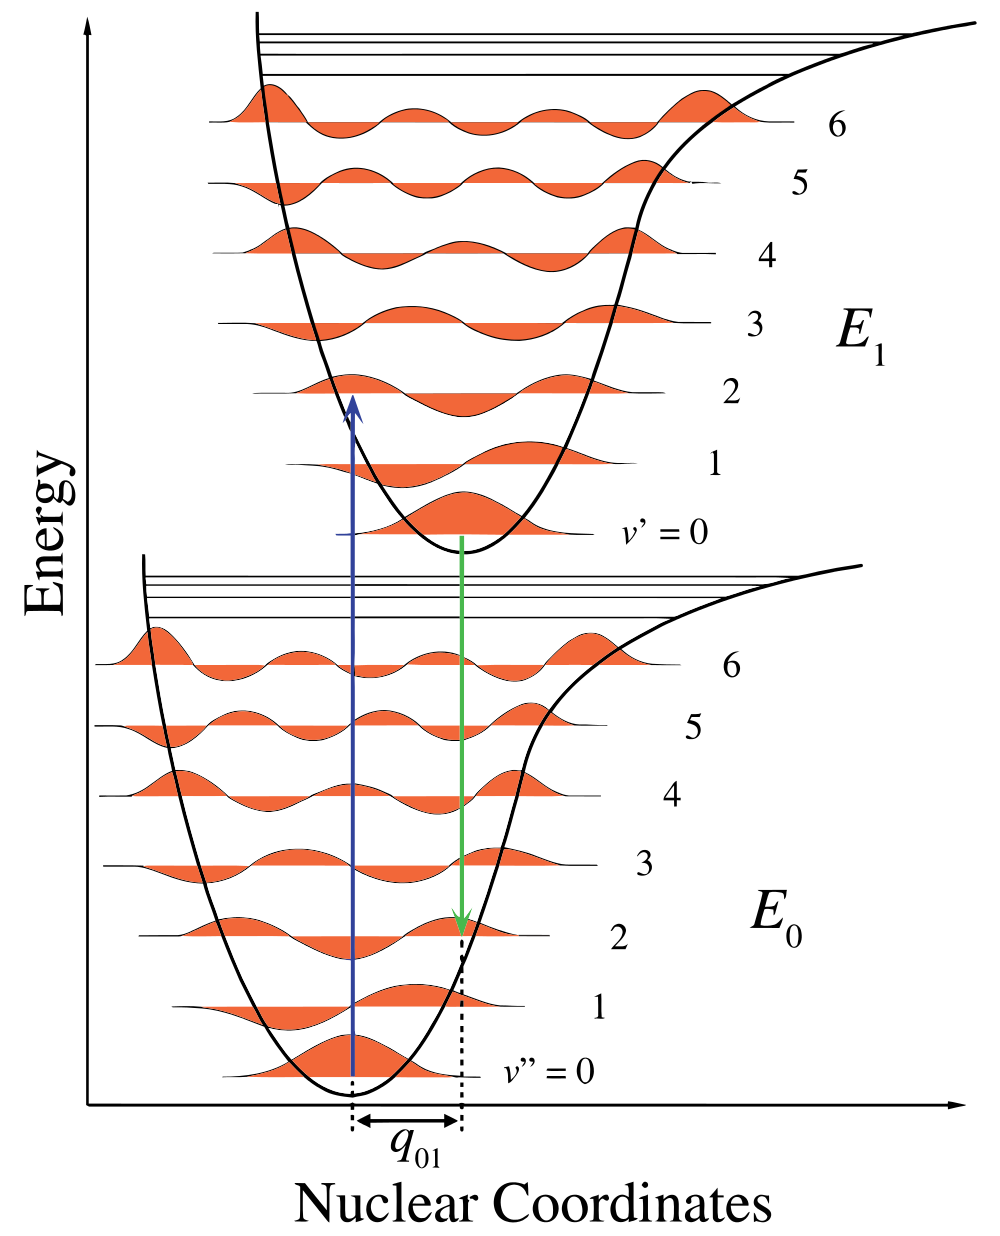
\includegraphics[width=0.5\textwidth]{fc.png}
\caption{Energy diagram for the FC principle. Since electronic transitions are much faster than the nuclear motions in a molecule, vibrational levels are favoured when they correspond to a minimal change in the nuclear distance (plotted on the x-axis). E.g. in this case, a transition is more likely to occur from the ground state to the excited state between the vibrational levels $v''=0$ to $v'=2$. After the vibrational energy is relaxed, a flourescent transition occurs from $v'=0$ down to $v''=2$. Image from Wikipedia.}
\label{fig:fc}
\end{figure}
Now, an absorption line in a molecule occurs more likely when the overlap between the wave functions of the vibrational states is larger, as can be seen in figure \ref{fig:fc}. Other transitions are also possible, with slightly different energies, but the lines correspond to the "center" of such a transition region.
\item We know the differential equation
\begin{equation}
\frac{\dif N}{\dif t} = -k N
\end{equation}
is solved by $N(t) = N_0 \cdot e^{-kt}$, where $N_0$ is the initial amount/concentration of e.g. carbon-14, $k$ is the decay constant and $t$ is time. From the exercise we know that $N(t)$ of carbon-14 is 28\% lower than in a living tree, i.e., $N(t) = 0.72 \cdot N_0$. We can thus write
\begin{align*}
0.72 N_0&= N_0 e^{-kt} \\
	0.72&= e^{-kt} \\
\ln(0.72)&= -kt \qquad \Rightarrow t = -\frac{\ln (0.72)}{k}
\end{align*}
Now, in order to determine $k$, we use the fact that after one half-life, the concentration has dropped to 50\%, i.e., if $t=\tau=\SI{5730}{\year}$. Then
\begin{align*}
0.5 N_0 &= N_0 e^{-k \tau} \\
\ln (0.5) &= - k \tau \\
k&= - \frac{\ln(0.5)}{\tau} \simeq \SI{1.21e-4}{\per\year}
\end{align*}
Plugging this back into our equation for $t$, we obtain
\[
t= - \frac{\ln(0.72)}{\SI{1.21e-4}{\per\year}} \simeq \SI{2714.9}{\year}
\]
\item One could view the decay of substance A as the creation of B and C happening at the same time. Therefore, the rate equation could be written as
\begin{equation}
\frac{\dif A}{\dif t} = k_A t = [k_B+k_C]t 
\end{equation}
If we suppose, for example, that $k_B = 0.4 k_A$ and $k_C = 0.6 k_A$, then the resulting concentration diagram looks roughly like figure \ref{fig:concentration_diagram_johannes}.
\begin{figure}[H]
\centering
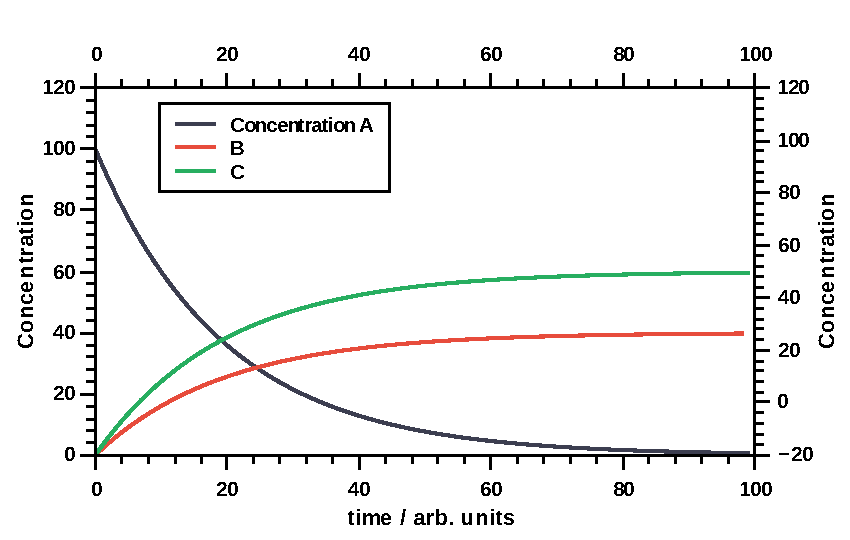
\includegraphics[width=0.8\textwidth]{question5-4d}
\caption{Concentration diagram for the reaction $A \to B + C$, where $k_B=0.4k_A$ and $k_C = 0.6k_A$ was chosen. The concentrations for B and C follow an inverse function of the exponential decay.}
\label{fig:concentration_diagram_johannes}
\end{figure}
\end{enumerate}



 \begin{thebibliography}{99}

  \bibitem{taube}
     \textsc{Henry Taube}, \textit{The Interaction of Manganic Ion and Oxalate. Rates, Equilibria and Mechanism}, J. Am. Chem. Soc., 1948, 70 (3), pp 1216–1220.

  \bibitem{manganese}
   \textsc{Krisztian A. Kovacs, Pal Grof, Laszlo Burai, and Miklos Riedel}, \textit{Revising the Mechanism of the Permanganate/Oxalate Reaction}, J. Phys. Chem. A 2004, 108, 11026-11031.

   \bibitem{k}
   \textsc{Uehiro Takashi, Taminaga Iwao, Yoshino Yukichi}, \textit{The Decomposition of the Oxalato Complex of Manganese(IV) in Oxalate Buffer Solutions}, Bulletin of the Chemical Society of Japan vol. 48(10), 2809-2812 (1975)

   \bibitem{skriptum}
Fortgeschrittenenpraktikum 2, \textit{Photometric measurements of the dissociation of manganese oxalate
}. 

\end{thebibliography}
\end{document}
